\newpage
\section{Conclusion}

This project has successfully developed and demonstrated a comprehensive investment model for optimizing 
technology asset deployment in integrated energy systems. The platform combines DC Optimal Power Flow (DCOPF) 
simulations with detailed investment analysis, providing valuable insights for decision-makers. Key 
achievements and conclusions include:

\begin{itemize}
    \item \textbf{Investment-Focused Optimization:} The platform effectively evaluates different technology 
    combinations through both technical and economic lenses. As demonstrated in the 9-bus case study, it can 
    simultaneously assess multiple aspects:
    \begin{itemize}
        \item Capital expenditure impacts on long-term profitability
        \item Operational costs and their influence on Net Present Value
        \item Storage sizing and its role in system economics
        \item Trade-offs between conventional and renewable technologies
    \end{itemize}
    
    \item \textbf{Economic Analysis Capabilities:} The model provides robust financial metrics for decision-making:
    \begin{itemize}
        \item Net Present Value (NPV) calculations across different time horizons (10, 20, 30 years)
        \item Annuity comparisons for assets with different lifetimes
        \item Sensitivity analysis to evaluate investment robustness and simulate load increase
    \end{itemize}

    \begin{figure}[H]
        \centering
        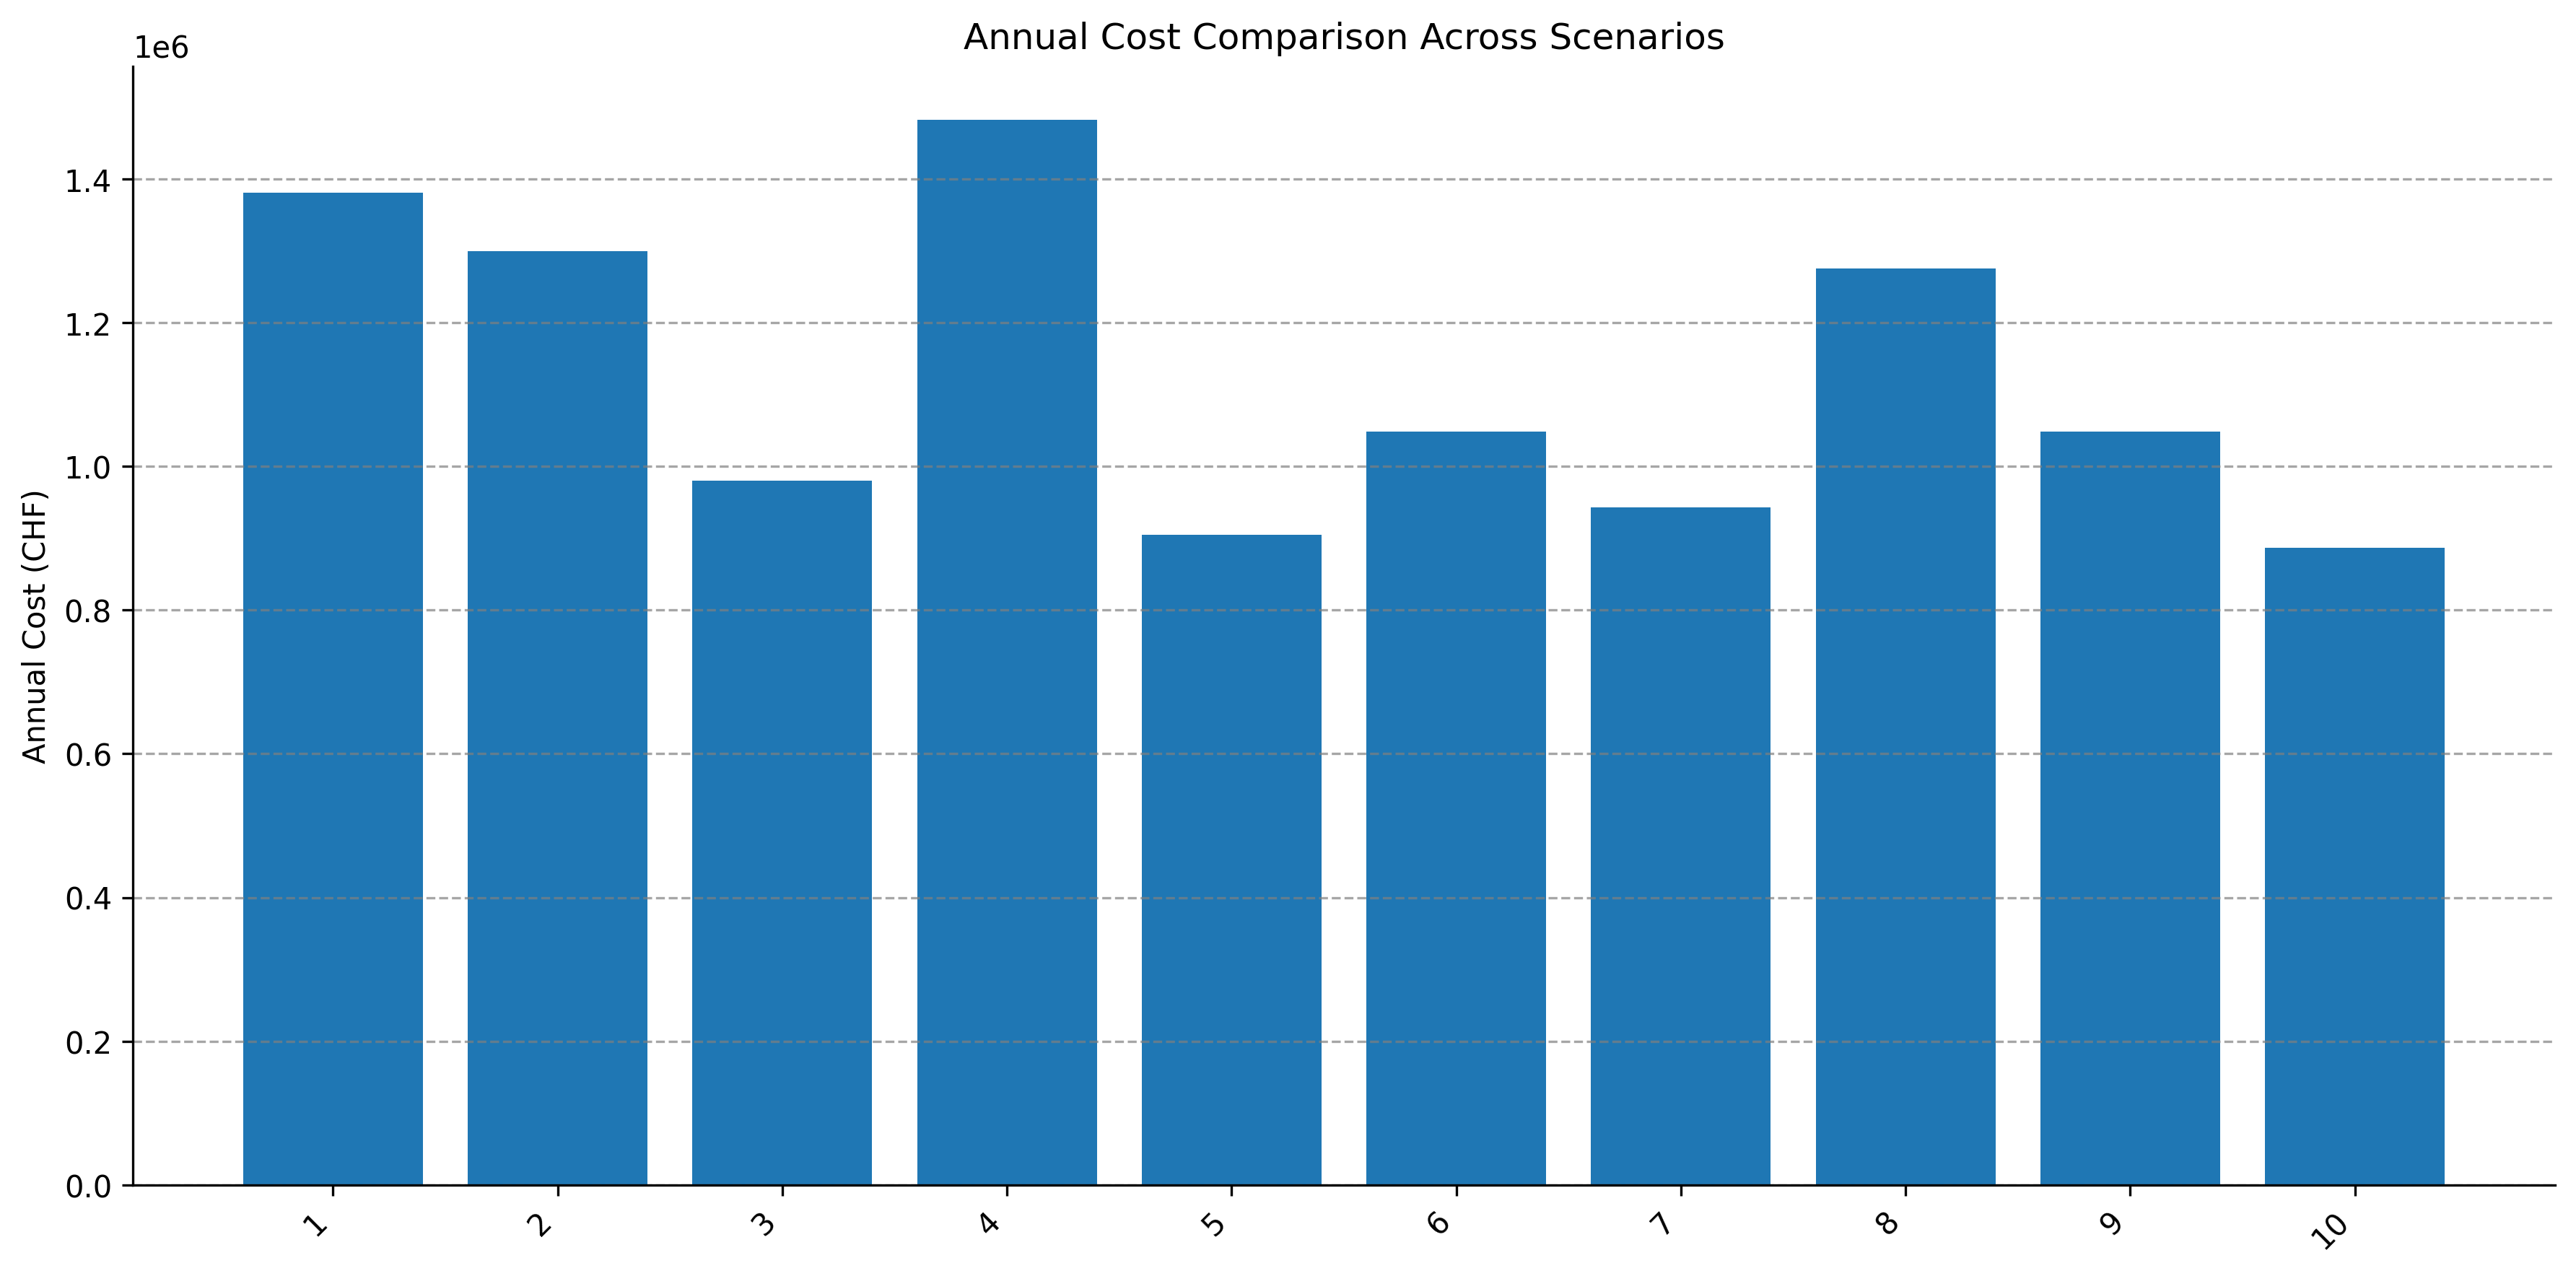
\includegraphics[width=0.6\textwidth]{images/global.png}
        \caption{Annuity comparison across scenarios}
        \label{fig:global_annuities}
    \end{figure}

    As shown in Figure~\ref{fig:global_annuities}, scenarios with balanced technology mixes (e.g., Scenarios 7 
    and 5) achieved the lowest annuities, around 1.35M CHF/year. These configurations with renewable generation 
    and appropriate storage, demonstrated the value of diversified technology portfolios. 
    
    In contrast, scenarios heavily dependent on gas generation or oversized storage (e.g., Scenario 4) showed 
    significantly higher annuities, reaching 1.84M CHF/year.
  \end{itemize} 

From a technical standpoint, the platform integrates DCOPF network constraints, multiple energy 
carriers, storage dynamics, and renewable generation variability. And, from a decision support standpoint, 
the system enables rapid scenario comparison, identifies cost drivers, assesses investment risks, and 
provides AI-enhanced analysis.

While the case study utilized a simplified 9-bus system, the methodology and platform have demonstrated their 
capability to handle the core requirements of investment decision support in energy systems. The results show 
that optimal technology selection depends on multiple factors, including:
\begin{itemize}
    \item Initial investment constraints
    \item Operational cost considerations
    \item Technology lifetime and replacement cycles
    \item System reliability requirements
\end{itemize}

Future development should be guided by use case requirements first. For utility-scale planning, priorities 
may include multi-carrier integration (gas, hydrogen) and sophisticated environmental assessments. For microgrid 
optimization, the focus should be on real-time pricing and enhanced storage modeling. For optimal energy system 
dimensioning, improving the framework to better determine optimal generator sizes based on demand profiles would 
be valuable. For renewable integration studies, improving sensitivity analysis capabilities and AI-driven scenario evaluation 
would be most valuable. 

Rather than pursuing all improvements simultaneously, development efforts should align with the intended 
application to ensure appropriate depth and accuracy where it matters most.The platform provides a solid foundation for investment decision-making in energy systems, balancing technical 
feasibility with economic viability. Its modular architecture allows for future extensions to address more 
complex scenarios and additional optimization objectives, such as emissions reduction, while maintaining its 
core strength in economic assessment and technology selection.

\newpage
\section*{Acknowledgements}

For the redaction of this report, I would like to acknowledge the use of artificial intelligence to improve
the clarity and structure of my sentences. The core observations, analyses, and personal reflections
are entirely my own, drawn from my experiences during the field trip and subsequent research. The
LLM usage was employed primarily for language refinement, code formatting, and orthographic corrections.
Its integration helped communicate complex concepts clearly and effectively.


\newpage
